\documentclass{sig-alternate}

% Include needed packages
\usepackage{graphicx}             	     % Needed for including EPS graphics
\usepackage{cite}                        % Needed for doing citations
\usepackage[noend]{algorithm,algorithmic}% Needed for algorithms	
\usepackage{subfigure}                   % Needed for subfigures

% Notation
\newcommand{\Orange}{\texttt{Orange}}
\newcommand{\GB}{\texttt{Goldenberry}}
\newcommand{\PBIL}{\texttt{PBIL}}
\newcommand{\UMDA}{\texttt{UMDA}}
\newcommand{\BMDA}{\texttt{BMDA}}
\newcommand{\PBILc}{\texttt{PBIL$_c$}}
\newcommand{\UMDAc}{\texttt{UMDA$_c$}}
\newcommand{\cGA}{\texttt{cGA}}
\newcommand{\EDA}{\texttt{EDA}}
\newcommand{\TILDA}{\texttt{TILDA}}
\newcommand{\CostFunction}{\texttt{CostFunctionBuilder}}
\newcommand{\BBTester}{\texttt{BlackBoxTester}}
\newcommand{\figref}[1]{\mbox{Figure \ref{#1}}}
\newcommand{\bs}{{\mathbf s}}
\newcommand{\bx}{{\mathbf x}}
\newcommand{\bw}{{\mathbf w}}
\newcommand{\bl}{{\mathbf l}}
\renewcommand{\bf}{{\mathbf f}}
\newcommand{\cB}{{\cal B}}
\newcommand{\Rdom}{\mbox{$\mathbb{R}$}}

\floatname{algorithm}{Algorithm}
\renewcommand{\algorithmicrequire}{\textbf{Requires:}}
\renewcommand{\algorithmicensure}{\textbf{Outputs:}}
\renewcommand{\algorithmicfor}{\textbf{repeat}}
\renewcommand{\algorithmicwhile}{\textbf{repeat until convergence}}
\renewcommand{\algorithmicdo}{\textbf{}}
\renewcommand{\algorithmiccomment}[1]{#1}
\algsetup{indent=1em}
\graphicspath{{figs/}}

\begin{document}
		\conferenceinfo{GECCO'13 Companion,} {July 6--10, 2013, Amsterdam, The Netherlands.}
		\CopyrightYear{2013}
		\crdata{978-1-4503-1964-5/13/07}
		\clubpenalty=10000
		\widowpenalty = 10000
%\title{Goldenberry: A suite of Estimation of Distribution Algorithms software components for the Orange platform}
%\title{EDA analysis with visual programming in Orange}
%\title{Goldenberry: A toolbox of visual EDA software components for Orange}
\title{Goldenberry: EDA Visual Programming in Orange}
%
\numberofauthors{2} 
\author{
\alignauthor
Sergio Rojas-Galeano\\
       \affaddr{Engineering School}\\
       \affaddr{District University of Bogota}\\
       \affaddr{Bogota, Colombia}\\
       \email{srojas@udistrital.edu.co}
\alignauthor
Nestor Rodriguez\\
       \affaddr{Engineering School}\\
       \affaddr{District University of Bogota}\\
       \affaddr{Bogota, Colombia}\\
       \email{nearodriguezg@correo.udistrital.edu.co}
}
\date{\today}
\maketitle

\begin{abstract}
\Orange~ is an open-source component-based software framework, featuring visual and scripting interfaces for many machine learning algorithms. Currently it does not support Estimation of Distribution Algorithms (\EDA) or other methods for black-box optimization. Here we introduce \GB, an \Orange~toolbox of \EDA~visual components for stochastic search-based optimization. Its main purpose is to provide an user-friendly workbench for researchers and practitioners, building upon the versatile visual front-end of \Orange, and the powerful reuse and glue principles of component-based software development. Architecture of the toolbox and implementation details are given, including description and working examples for the components included in its first release: \cGA, \UMDA, \PBIL, \TILDA, \UMDAc, \PBILc, \BMDA, \CostFunction~and \BBTester. 

\GB~is open-source and freely available at: \\\texttt{\mbox{~~~~~~~}http://goldenberry.codeplex.com}.
\end{abstract}

\category{D.2.6}{Software}{Software Engineering}[Programming Environments]
\category{I.2.8}{Computing Methodologies}{Artificial Intelligence}[Problem Solving, Control Methods and Search]
%\terms{Algorithms, Design, Experimentation.}

%\keywords{EDA, data mining software, component-based evolutionary software systems}
\keywords{Component-based evolutionary software systems; EDAs}

\section{Introduction}
Visual environments for machine learning (e.g. Clementine or SPSS Modeler\cite{ibm2012}, Weka\cite{Hall2009}, RapidMiner\cite{Mierswa2006}) provide graphical workbenches to conduct user-friendly data analysis. Instead of scripting commands in an imperative computer language, users are able to graphically sketch processing units and interactions that are needed to run said analysis. \Orange~is one of such open-source visual frameworks, originally proposed for functional genomic analysis \cite{Curk2005}. It has been progressively enriched with additional visual software components (\textit{widgets}) for several machine learning tasks. It is known that many of these tasks can be casted as, or make use of, optimization problems in their underlying machinery (regression analysis, regularization, clustering, feature selection); however as far as we know, to this day \Orange~does not include a set of tools available to model explicit optimization problems within the context of machine learning analysis. The latter is precisely the motivation behind the software system we introduce in this paper: \mbox{\GB}, a supplementary machine learning and evolutionary computation suite for \Orange.

The software was built by taking advantage of three interesting features in \Orange: (i) its versatile visual front-end; (ii) the powerful reuse and glue postulates of component-based software development in which it is based; and (iii) its conformity to the \textit{open/closed} principle of object-oriented programming through an scripting interface to Python. We reasoned that such features would be advantageous for extending its functionality to the realm of optimization problems. Since our research group has been recently working on stochastic-search-based optimization, particularly in the field of Estimation of Distribution Algorithms (\EDA\cite{Larranaga01, Pelikan06}), a decision was made to start off the project in its first stage by focusing on this kind of algorithms. As a result, the first release of \GB~comprises a set of \EDA~components (\cGA\cite{Harik99}, \UMDA\cite{Muhlenbein97}, \PBIL\cite{Baluja95}, \TILDA\cite{Rojas2012}, \PBILc\cite{Sebag98}, \UMDAc\cite{Larranaga02}  and \BMDA\cite{Pelikan99}) and a set of utility components (\CostFunction~and \BBTester) that we shall describe in the following sections. The second stage of the project is currently under development; it will comprise other black-box optimization techniques and also additional meta-heuristics and machine learning components. 

The paper describes a general depiction of the software architecture, and provide working examples of its operation using standard benchmark and custom optimization problems. The latter was made possible by using the built-in cost functions or the free-text Python input mode from the \CostFunction~component, which are convenient design features allowing this suite to be applied over a wide range of discrete and continuous optimization domains. 
\GB~is also open-source and is freely available at: \\ \mbox{~~~~~~~}\texttt{http://goldenberry.codeplex.com}

\noindent For download instructions please refer to the Appendix.

\section{The software at a glance}
\GB~was built as a suite of \emph{widgets} for \Orange. Widgets are visual elements that can be dragged onto the \Orange~visual programming board, also known as \emph{canvas}. Furthermore, widgets provide a set of input/output interfaces that encapsulate related services; many widgets collaborate to perform a given task. ``Programming'' in the canvas amounts to manually wiring up the appropriate interfaces between widgets. An example of a \GB~program to optimize a cost function using three different \EDA~widgets is shown in \figref{fig:canvas}. In that program, widgets are the components or processing units needed to perform the optimization task.  Rather than depicting a \emph{dataflow} between these components, connections represent provision and consumption of services encapsulated as objects, which are associated with each input/output interface. For instance, in this program the \cGA, \PBIL~ and \UMDA~widgets require a function to be optimized that is provided by the \mbox{\CostFunction} widget through three instances of the \texttt{CostFunction} object, one per \EDA, each in charge of keeping statistics of the number of function evaluations and running times. The \EDA~components are responsible of setting up the parameters of their corresponding algorithm and of providing a ready-to-use \texttt{Optimizer} that is in turn, consumed by the \BBTester. The latter is in fact responsible of orchestrating the execution of these \texttt{Optimizer}s, that is, of running each \EDA~algorithm (whose parameters, including cost function, must have been already defined and provided in their output interfaces before execution begins) and also of collecting and visualizing the final results. Parameter settings and data presentation are embodied within the the graphical user interface of the widgets, as we shall depict in Section \ref{sec:components} and \ref{sec:experiments} (also \figref{fig:cga_run} to \figref{fig:custom}). Intuitively, this programming paradigm is very much the same as building a hardware apparatus: the user first gather, connect and set-up the required units before switching-on the resulting device.  


\section{Architectural view}

\subsection{General design considerations}
\label{sec:patterns}
The following software patterns were taken into account during the conception of \GB:

\begin{itemize}
	\item A \emph{layering} pattern\cite{Buschmann96} was applied in order to decouple the algorithmic logic of the components from their user interface (widgets); thereby all the implemented algorithms can be used and integrated in plain Python scripts or using the command-line. 
	\item A \emph{template method} pattern\cite{GangOfFour} was used by identifying commonalities of the different \EDA~approaches. In this way a generic abstraction of an \EDA~procedure was defined; concrete details of implementation were deferred to each particular algorithm.  A unified \EDA~framework was achieved.
	\item A \emph{responsibility splitting} pattern\cite{Bachmann07} was utilised in \EDA~optimisers so as to separate the search metaheuristic from the probability estimation technique. Therefore probability models were made reusable among multiple \EDA s (those included in this and future releases).
	\item A \emph{dynamic binding}\cite{Bachmann07} together with an \emph{interpreter} pattern\cite{GangOfFour} were applied in order to allow the user to provide customised cost functions at runtime, in the form of Python-like scripts.
\end{itemize}

The application of such patterns guided the resulting design of the software, as described in the remainder of this section.


\begin{figure}[h]
	\centering
	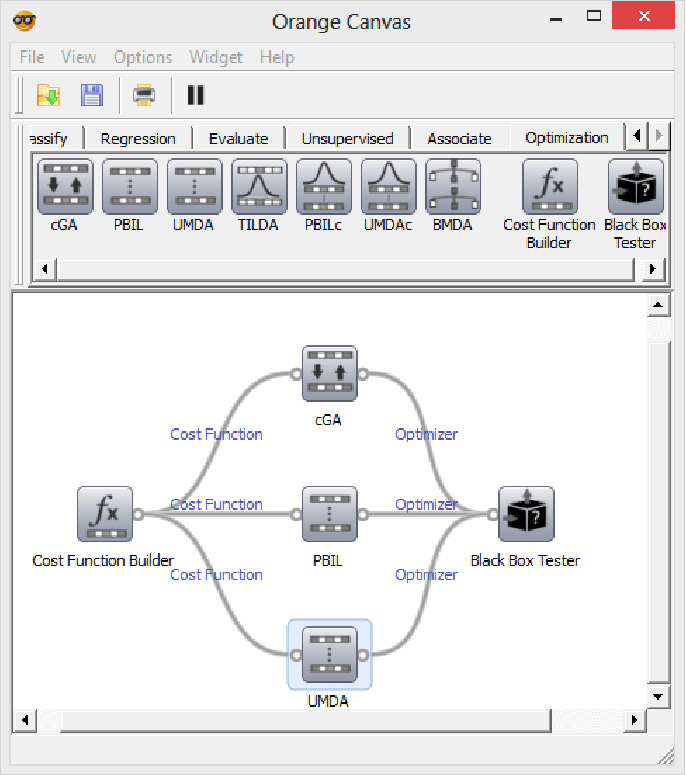
\includegraphics[width=1.0\columnwidth,height=.4\textheight]{canvas} 
	\caption{{\small A \GB~program in the \Orange~canvas.}}
	\label{fig:canvas}
\end{figure}

\begin{figure}[h]
	\centering
	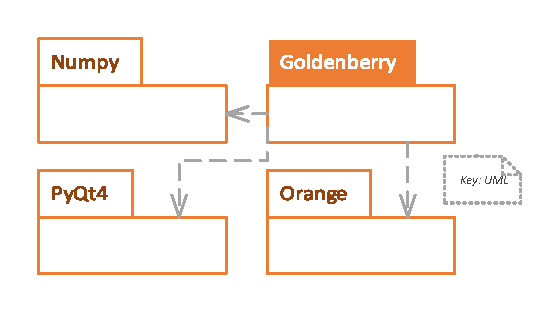
\includegraphics[scale=.75]{context} 
	\caption{The context diagram of \GB.}
	\label{fig:context}
\end{figure}

\begin{figure}[H]
	\centering
	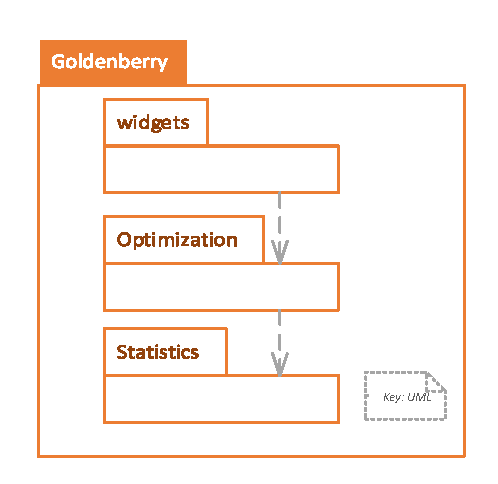
\includegraphics[scale=.75]{modules} 
	\caption{The three basic modules in \GB.}
	\label{fig:modules}
\end{figure}


\begin{figure*}
\centering
	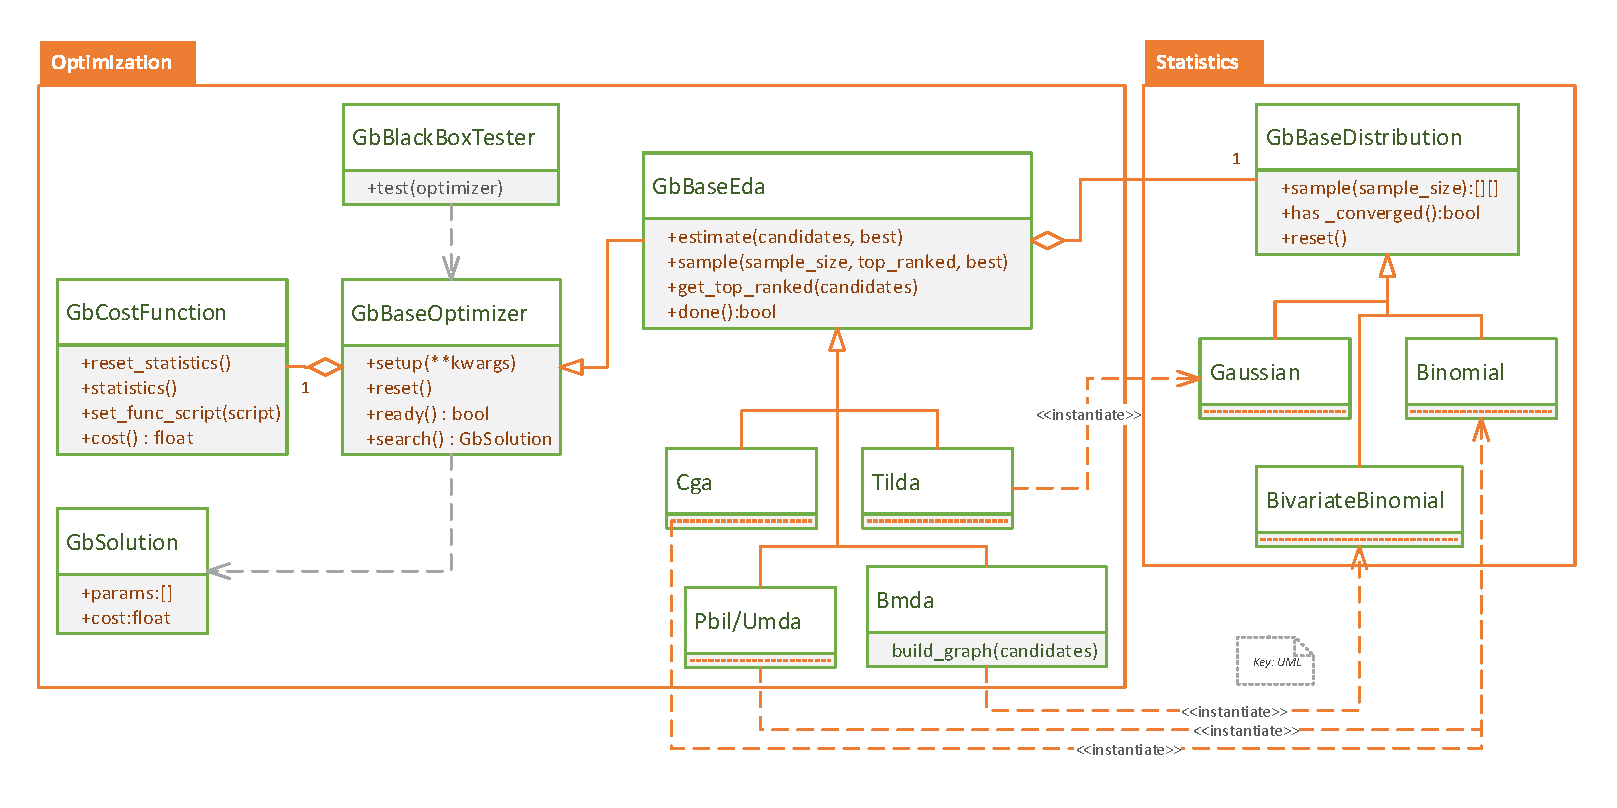
\includegraphics[scale=.65]{modules_drilldown} 
	\caption{Decomposition view of \GB~modules.}
	\label{fig:modules_drilldown}
\end{figure*}

\subsection{Architecture packages}
Widgets are actually visual wrappers for software components written in the Phyton scripting feature provided by \Orange. Implementation of any widget or suite of widgets require the use of the \Orange~core library, the \texttt{PyQt4} library for user-interface designing tools and optionally, the \texttt{NumPy} library for additional scientific computation support (\texttt{PyQt4} and \texttt{NumPy} are standard libraries of the Python programming language). Therefore, the top-level organization of the \GB~suite of widgets is illustrated in the context diagram of \figref{fig:context}.  

The internal architecture of the current release is shown in the module diagram of \figref{fig:modules}. Three modules were developed. The \texttt{widgets} modules are the visual wrappers for the suite of \GB~components. The \texttt{Optimization} module includes objects and routines needed to implement the \EDA~components; this is the core module of the suite. Finally, \texttt{Statistics} is a utility module to allow modelling of some probability distributions used by the \EDA~algorithms.

\section{Structural view}
A decomposition view of the \texttt{Optimization} and \texttt{Statistics} modules including object classes and dependencies, is shown in the class diagram of \figref{fig:modules_drilldown}. It is expected that the modular design proposed here, would allow for new or customized \EDA~algorithms, probability distributions or other stochastic-search optimizers, to be added to the toolbox as extensions of such architecture. This would be one of the advantages of observing the software patterns earlier mentioned in Section \ref{sec:patterns}.

\subsection{Base classes}
A core class \texttt{GbBaseOptimizer} was designed as an abstract class representing any black-box optimization algorithm (see \figref{fig:modules_drilldown}). The optimizer uses a \texttt{GbSolution} object, which holds the values of the parameters or variables in an arbitrary solution to a given problem (the vector \texttt{params[]}); it also holds its associated cost. The optimizer additionally encapsulates a \texttt{setup()} method to initialize its running parameters (e.g. problem size or number of variables, maximum number of evaluations, etc.) and the \texttt{reset()} method to set up the optimizer for a new run. The key method \texttt{search()}, defines the actual optimization algorithm which returns a best found solution; \texttt{ready()} is a checkpoint method to validate readiness of the optimizer to start the search.

A given candidate solution is evaluated with the \texttt{cost()} method from the \texttt{GbCostFunction} class (in the evolutionary computation literature this would be equivalent to computing the \emph{fitness} of a candidate). The routine to evaluate the function is defined via the \texttt{set\_func\_script()} method. Furthermore, this class also includes a method to keep track of \texttt{statistics()}, such as the number of cost function evaluations or max/min/mean cost values; the {\texttt{reset\_statistics()}} method clears up the statistics working memory.\\

\subsection{EDA classes}
In the current release \GB~provides implementation of only \EDA-type optimizers. Other black-box optimization techniques would be added in the near future. Hence, a specialized abstract class \texttt{GbBaseEda} was derived from \texttt{GbBaseOptimizer} (see \figref{fig:modules_drilldown}). This class defines the two distinctive methods of any \EDA: \texttt{estimate()} as the mechanism that builds up its probabilistic model, and \texttt{sample()} as the algorithm to generate new candidate solutions from that model. Two additional methods were designed: \texttt{get\_top\_ranked()} selects the promising candidates from where the probability model estimation is updated; and \texttt{done()}, which checks for convergence of the estimated model. These are the methods that would be iteratively executed during a run of the \texttt{search()} method from the parent class.

A particular implementation of the \texttt{GbBaseEda} class aforementioned, determines a type of \EDA~algorithm that would be used as optimizer. \GB~features a number of concrete \EDA~implementations, including univariate algorithms such as \cGA, \TILDA, \PBIL~and \UMDA~(discrete and continuos-domain variants for the last two), and also a bivariate algorithm, the \BMDA. The latter extends the base class with an additional method \texttt{build\_graph()} to model pairwise dependencies between problem variables. This assortment of algorithms was chosen so as to incorporate techniques using both univariate and bivariate probability distribution approaches. In the first release of the software we emphasised in univariate versions due to their algorithmic simplicity; nonetheless, future releases will build upon these algorithms and contemplate higher-order \EDA  s using tree-based, Bayes and dependency networks techniques.

For illustration purposes, we shall now outline some of the Python scripts implementing these classes. Firstly, let us recall the \textit{Population-Based Incremental Algorithm} (\PBIL)\cite{Baluja95}. The aim of this algorithm is to discover a real-valued probability vector from which a population of competent  binary candidate solutions can be sampled. The algorithm starts-off with a random-valued vector; then, the vector is iteratively sampled in order to refine the model using the most promising solutions from the sample and an \emph{incremental learning} re-estimation rule, until the vector converges to a fixed distribution. Our rendering of this procedure is shown in Algorithm \ref{alg:PBIL}, were a vectorized operation mode was assumed.

\begin{algorithm}[H]
	\caption{\PBIL} 
	\small
	\begin{algorithmic}
	\REQUIRE Cost function $\mathsf{fitness}(\cdot)$, binomial distribution model $\cB(\boldsymbol \theta)$ with parameters $\boldsymbol \theta\in \Rdom^d$, learning rate $0 \le \eta \le 1$
	\ENSURE Solution $\bs \in \Rdom^d$
		\STATE Initialize $\boldsymbol \theta$ and $\bs$ with random values in $[0,1]^d$
		\WHILE{}
			\STATE Sample $n$ candidates from model: $P \sim \cB(\boldsymbol \theta)$ 
			\STATE Assess fitness of candidate population: $\bf = \mathsf{fitness}(P)$
			\STATE Choose $m$ candidates: $S = \{\bx_i \in P : f_i \in \textnormal{ top-$m$-ranked}\}$
			\STATE Re-estimate model: $\boldsymbol \theta = (1-\eta)\boldsymbol \theta + \eta\tfrac{1}{m}\sum_i{\bx_i}, \quad\bx_i \in S$
			\STATE Update solution: $\bs\!=\!\mathsf{argmax}(\mathsf{fitness}(\bs),\mathsf{fitness}(S^{top}))$
		\ENDWHILE
	\end{algorithmic}  
	\label{alg:PBIL}
\end{algorithm}

In \GB, the \PBIL~widget defines a class \texttt{Pbil} which overrides the \texttt{initialization()} and \texttt{estimate()} methods according to the previous algorithm. Thus, \PBIL~is fully implemented as the following class script (notice that the \texttt{average} vectorized auxiliary operation from the   \texttt{NumPy} library (\texttt{np}) is used):

\begin{verbatim}
class Pbil(GbBaseEda):
 def initialize(self):
   self.distr=Binomial(self.var_size)    

 def estimate(self, top_ranked, best):
   self.distr.p=self.distr.p*(1-self.learning_rate)
      + self.learning_rate * np.average(top_ranked)
\end{verbatim}

The small size of the script is due to the fact that many algorithmic details have been inherited from the parent class, \texttt{GbBaseEda}, because they are common to most of other \EDA s. For example, the parent class defines the initialization of parameters such as \texttt{sample\_size}, \texttt{pop\_size} (size of the population), \texttt{selection\_rate} (percentage of top-ranked selected candidates), and \texttt{max\_evals} (limit on the number of cost function evaluations allowed on an entire search). Other common features such as the \texttt{sample()} method (which delegates this task to the respective probability model), the \texttt{get\_top\_ranked()} method to select the most promising candidates from the sample, and the \texttt{search()} method itself, are defined in this abstract class. Its script is partially shown below.

%class GbBaseEda(GbBaseOptimizer):
%...
%   def setup(self, var_size=10, pop_size=20, 
%   max_iters=None, max_evals=None, 
%   selection_rate=50, learning_rate=1.0, **kwargs):
%       self.sample_size = pop_size/2
%       self.__dict__.update(**kwargs)
%       self.reset()
%       self.initialize()

\begin{verbatim}
class GbBaseEda(GbBaseOptimizer):
...
 def sample(self, sample_size, top_ranked, best):
    return self.distr.sample(sample_size)

 def get_top_ranked(self, candidates):
    fits = self.cost_func(candidates)
    index = np.argsort(fits)
     [:(self.cand_size*self.selection_rate/100):-1]
    return candidates[index], 
     bSolution(candidates[index[0]],fits[index[0]])
... 
 def search(self):
     if not self.ready():
      raise Exception("Optimizer not ready.")
     best = GbSolution(None, float('-Inf'))
     top_ranked = None
     while not self.done():
         candidates=self.sample(self.sample_size, 
                                top_ranked, best)
         top_ranked, winner = 
                  self.get_top_ranked(candidates)
         self.estimate(top_ranked, best)          
         if best.cost < winner.cost:
             best = winner
         self.iters += 1
     return best

 @abc.abstractmethod
 def estimate(self, candidates, best):
     raise NotImplementedError()
\end{verbatim}

It can be seen in the previous code that the implementation of \texttt{estimate()}, the estimation of distribution method, is deferred to the specific \EDA~class, as it was the case of the \PBIL~component. 

Now let us complete the illustration by mentioning another well-known \EDA, the \textit{Compact Genetic Algorithm} (\cGA)\cite{Harik99}. The algorithm is similar in fashion to \PBIL, the main difference being that it operates in a \textit{compact} mode, that is, instead of estimating the distribution from a batch of many candidates (population), the algorithm works by sampling two candidates at a time and using them to incrementally build the estimation. The pseudo-code of this procedure is thus shown in Algorithm \ref{alg:cGA}, which again is our rendition of the original, written in vectorized operation mode.

\begin{algorithm}[H]
	\caption{\cGA} 
	\small
	\begin{algorithmic}
	\REQUIRE Cost function $\mathsf{fitness}(\cdot)$, binomial distribution model $\cB(\boldsymbol \theta)$ with parameters $\boldsymbol \theta\in \Rdom^d$
	\ENSURE Solution $\bs \in \Rdom^d$
		\STATE Initialize $\boldsymbol \theta$ and $\bs$ with random values in $[0,1]$
		\WHILE{}
			\FOR{$n$ \textbf{times}}
				\STATE Sample $2$ candidates from model: $\{\bx_1,\bx_2\} \sim \cB(\boldsymbol \theta)$
				\STATE Rank them: $ \{\bw, \bl\}=\mathsf{compete}(\mathsf{fitness}(\bx_1), \mathsf{fitness}(\bx_2))$ 
				\STATE Re-estimate model with winner and loser: $\boldsymbol \theta\!=\!\boldsymbol \theta+ \tfrac{1}{n}(\bw\!-\!\bl)$
				\STATE Update solution: $\bs = \mathsf{argmax}(\mathsf{fitness}(\bs),\mathsf{fitness}(\bw))$
			\ENDFOR
		\ENDWHILE
	\end{algorithmic}  
	\label{alg:cGA}
\end{algorithm}

The \cGA, as implemented in full in \GB, is shown in the script below. 

\begin{verbatim}
class Cga(GbBaseEda):
   def initialize(self):
       self.distr=Binomial(self.var_size)
       self.learning_rate=1.0/float(self.pop_size)
       self.sample_size=2
   
   def estimate(self, (winner, loser), best):
       self.distr.p = 
         np.minimum(np.ones((1, self.var_size)), 
           np.maximum(np.zeros((1, self.var_size)), 
           self.distr.p + 
  (winner.params-loser.params)*self.learning_rate))

   def get_top_ranked(self, candidates):
       costs = self.cost_func(candidates)
       maxindx = np.argmax(costs)
       winner = GbSolution(candidates[maxindx],  
                           costs[maxindx])
       loser = GbSolution(candidates[not maxindx], 
                          costs[not maxindx])
       return  (winner, loser), winner      
\end{verbatim}

The algorithm is initialized with the following settings: a binomial univariate probability model the size of the number of variables; learning rate of $1/n$ (where $n$ is the population size); and sample size of two, because of its  \emph{compact} style. The \texttt{estimate()} method is overridden to account for a compact learning rule, using two competitors; here again, the auxiliary  \texttt{NumPy} library is used (\texttt{np}). The \texttt{get\_top\_ranked()} is overridden accordingly, to return the winner and loser of the contest as the top-ranked set.
 
\subsection{Statistics classes}
The classes comprising this module were designed to account for the mechanisms needed to modeling probability distributions. A \texttt{GbBaseDistri\-bution} is defined encapsulating a \texttt{sample()} method, a \mbox{  }  \texttt{has\_converged()} validation method, and a \texttt{reset()} method for randomly initializing the parameters of the probability model (see \figref{fig:modules_drilldown}). Currently four probability distributions are implemented: \texttt{Bino\-mial}, \texttt{Gaussian}, \texttt{TruncatedGaussian} and \texttt{BivariateBinomi\-al}. Most of the functionality of these classes were implemented using standard \texttt{NumPy} routines such as generation of normally independent distibuted random vectors, and element-wise vector operators (details omitted). 

%For the sake of illustration, the full script implementing the class \texttt{Gaussian} is depicted below. It can be seen that the \texttt{NumPy} library (\texttt{np}) is used again for standard routines such as generation of normally independent distibuted random vectors, or to initialize all-ones or all-zero vectors. 

%\begin{verbatim}
%class Gaussian(GbBaseDistribution):   
%...
%   def sample(self, sample_size):
%       return np.random.randn(sample_size, self.n)*
%          self.stdevs + self.means

%   def has_converged(self):
%       return (self.stdevs < 0.01).all()

%   def reset(self):
%       self.means = np.zeros(self.n)
%       self.stdevs = np.ones(self.n)  
%        
%\end{verbatim}


\section{Components view}
\label{sec:components}
\figref{fig:components} shows the components view of the toolbox. For illustration purposes only two \EDA~components are shown: \cGA~for discrete domains and \TILDA~for continuous-valued domains (we recall the other implemented components are: \PBIL, \UMDA, \PBILc, \UMDAc, \BMDA). 

\subsection{The EDA components}
Any of these components internally consists of a collaboration between an \EDA~algorithm and a probability model (e.g. \cGA~uses a binomial distribution, \TILDA~uses a Gaussian distribution, and so on). Each \EDA~component exposes two interfaces. The first interface requires a \texttt{GbCostFunction} object that is able to evaluate the cost function on a given candidate solution, and also is able to trace statistics of the total number of evaluations made by the \EDA. The second interface provides a \texttt{GbBaseOptimizer} object, initialized and ready to run a stochastic search to optimize the cost function. 

These components are at the end of the day deployed as widgets in the \Orange~canvas, under a new toolbar named ``Optimization'' (see again \figref{fig:canvas}). The user interface of these widgets consists of a setup/results window. In there, parameters settings are applied to the \EDA~component and optimization results are displayed in an output text box after execution of the algorithm. An example of the user interface for the \cGA~widget, applied to solve the classical \texttt{OneMax} problem with 100 variables, using a population size of 30, and 1000 maximum number of evaluations, is shown in \figref{fig:cga_run}. 

\begin{figure}[H]
	\centering
	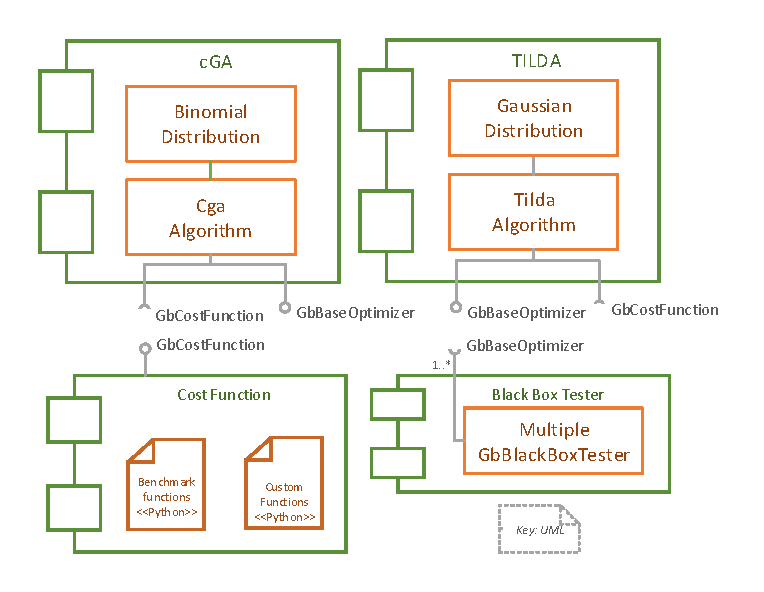
\includegraphics[scale=.7]{components} 
	\caption{The components diagram of \GB.}
	\label{fig:components}
\end{figure}

\begin{figure}[H]
	\centering
	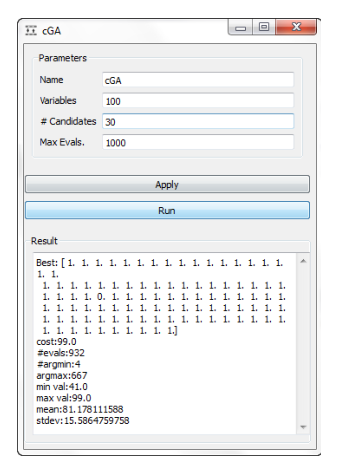
\includegraphics[scale=1.12]{cga_run} 
	\caption{User interface of the \cGA~widget.}
	\label{fig:cga_run}
\end{figure}

\begin{figure}
	\centering
	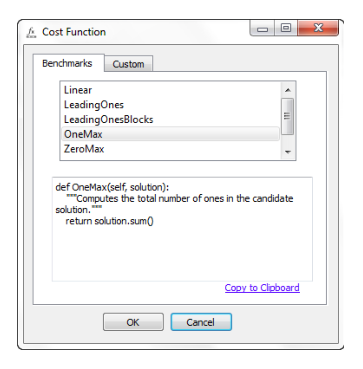
\includegraphics[scale=1.1]{onemax_costfun} 
	\caption{The benchmark input mode of the \CostFunction~component. Here the well-known \texttt{Onemax} problem is chosen.}
	\label{fig:onemax_costfun}
\end{figure}

\begin{figure}[H]
	\centering
	\subfigure[]{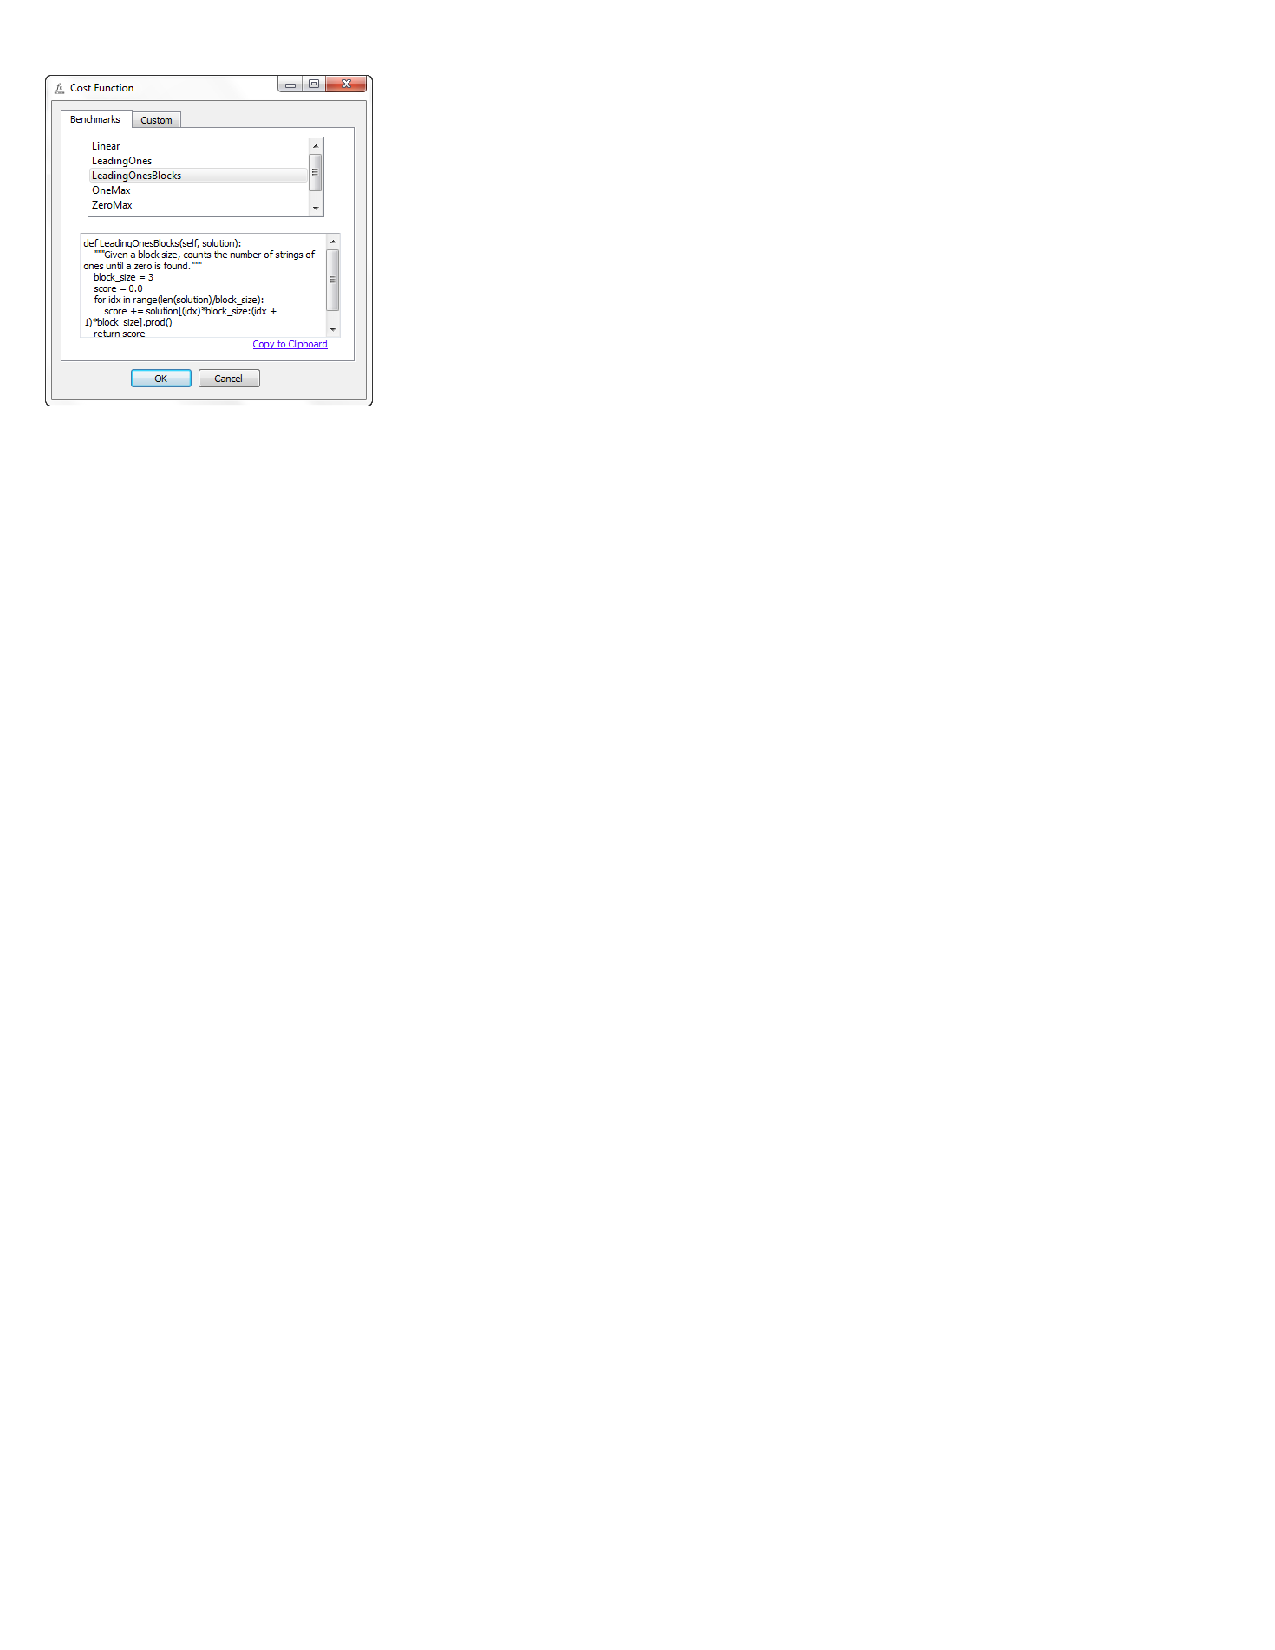
\includegraphics[scale=1.1]{onesblock_costfun}
	\label{fig:custom1}}
	\subfigure[]{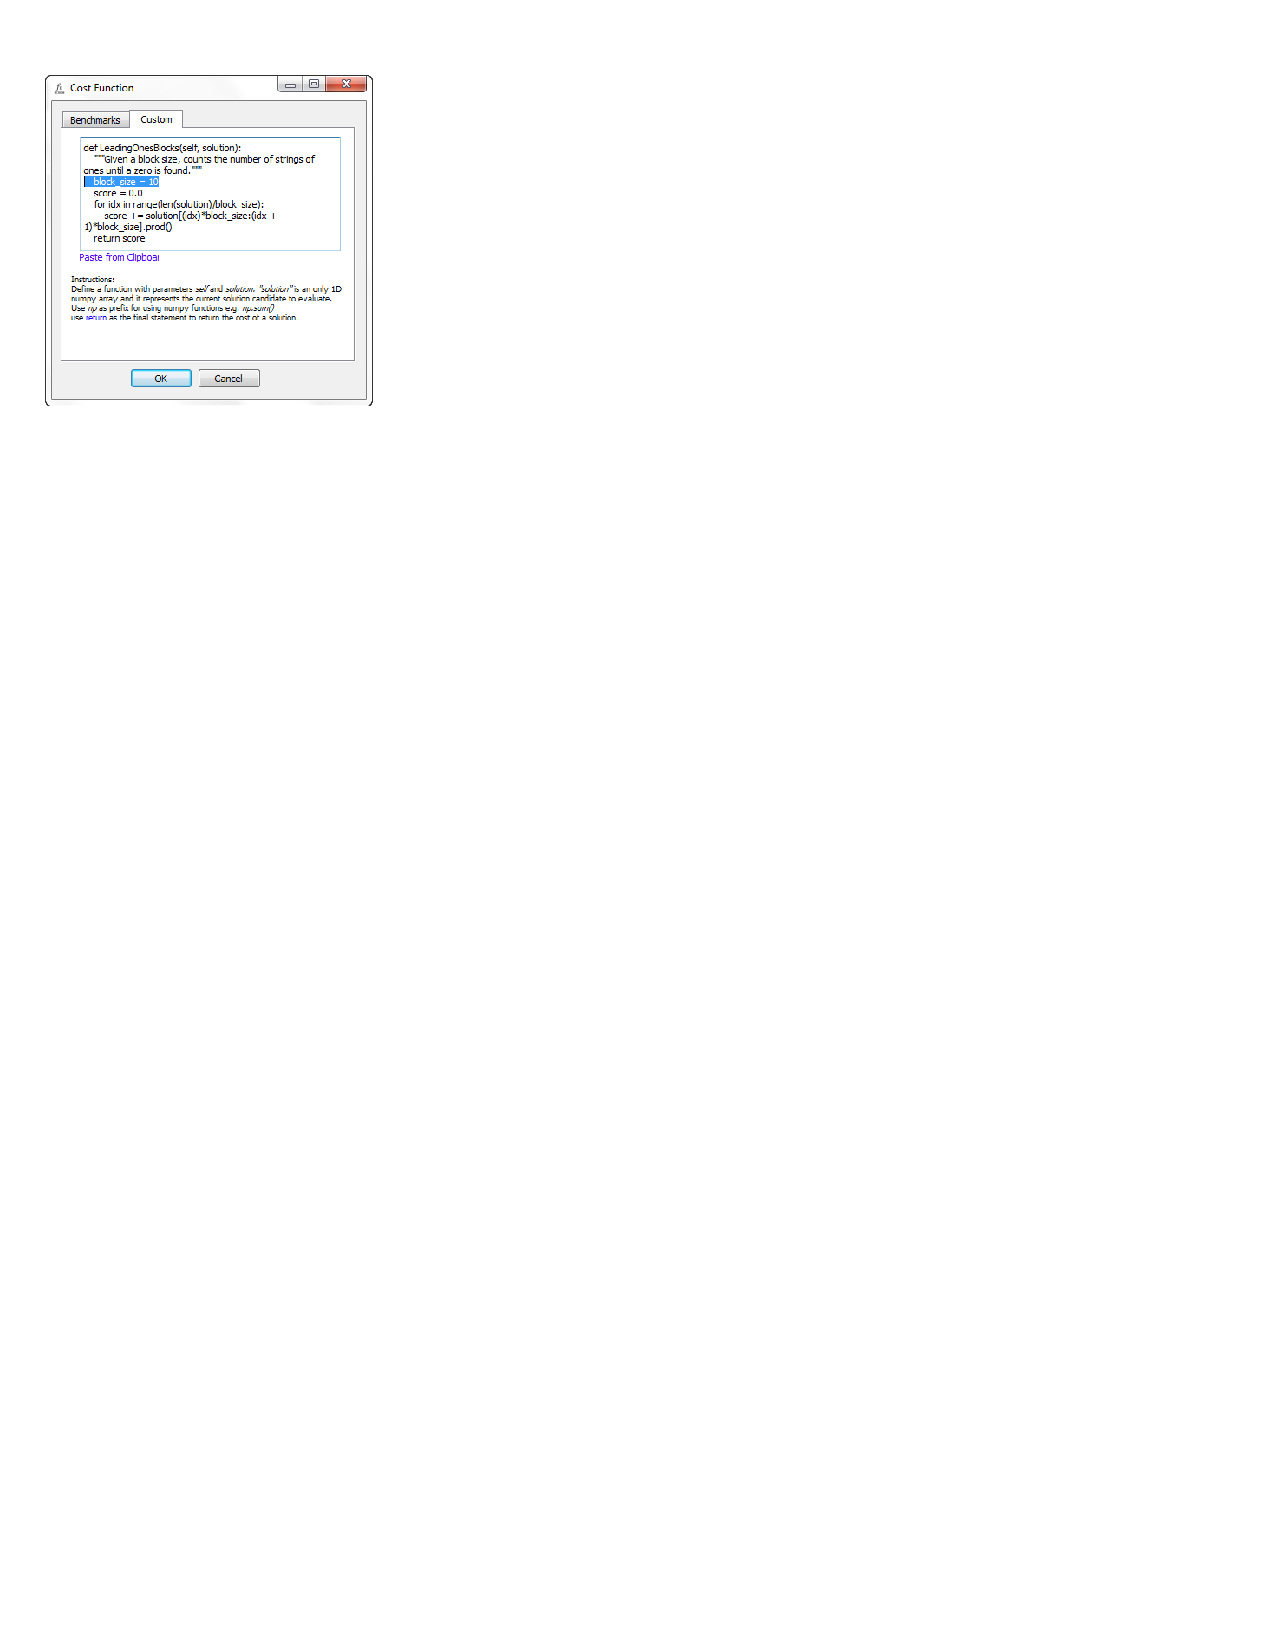
\includegraphics[scale=1.1]{custom_costfun} 
	\label{fig:custom2}}
	\caption{How to customize a built-in bechmark function: \subref{fig:custom1} A benchmark function is chosen and its code is copied into the clipboard; \subref{fig:custom2} the code is pasted in the ``Custom'' tab and edited as required.}
	\label{fig:custom_costfun}
\end{figure}

\subsection{The Cost Function Builder component}
This component enables the user to define the cost function for the optimization problem. It provides two input modes to setup such a function. In the first mode, a set of ready-to-use built-in benchmark functions are listed to the user as it is illustrated in \figref{fig:onemax_costfun}. This mode appears on the ``Benchmarks'' tab of the \CostFunction~user interface. The user chooses a function name, and then the Python script implementing the function is shown in the underlying text box; the box is read-only, so the code can not be edited but can be copied into the clipboard. The benchmark functions were taken from those suggested in \cite{Luke2009}.

The second mode consists of a free-text input box for writing up any customized cost function in the Python language. This mode appears on the ``Custom'' tab of the \CostFunction~~user interface. Custom functions must be written complying with the following Python-style signature: \\\\
\texttt{def \emph{yourcustomfunctionname}(self, solution):}\\ 
\texttt{...}\\
\texttt{return \emph{computedcostofsolution}}\\

An arbitrary routine to evaluate the given \texttt{solution} (a \texttt{NumPy} 1D vector array with the values of that solution to the problem variables) must be defined in order to compute its associated cost. For example, if the user wants to define a customized version of the benchmarks built-int functions, he or she may copy to the clipboard its original code, then paste it in the ``Custom'' tab and make the necessary adjustments (see \figref{fig:custom_costfun}). Alternatively the user may write up his cost function code from scratch, to meet his particular problem needs. We remark that this a is non-intrusive input mode, meaning that the user-written-code is bind to the \GB~components in run time; no additional intervention has to be done in the source code of the software. We anticipate this feature would extend the usability of the \EDA~components to a wide range of discrete and continuous optimization problem domains.

\subsection{The Black-Box Tester component}
This component was designed to allow the user to run and compare execution of different algorithms or algorithm configurations over the same cost function, in one experiment with several repetitions. The number of repetitions is set as an input parameter for this component. Another interesting functionality of the \BBTester~is that it is able to collect outputs of all the optimizer components provided as inputs, and display summarized statistics, and also details of the different runs and repetitions. The user interface of the widget associated to this component will be used to display results for the working experiments reported in the next section.

\section{Goldenberry at work}
\label{sec:experiments}
In this section we show how to use the developed components to solve optimization problems defined as minimization of a cost function. We carried out experiments using benchmark and customized cost functions. Other uses in machine learning can be also envisioned (see for example the discussion in Section \ref{sec:conclusions}).

The results of these experiments are shown next. It is worth to remark that previous to deployment, additional validation for the algorithmic machinery of each of the \texttt{Golden\-berry} components was carried-out using a carefully designed set of unit tests (omitted because of space limitations). The program shown in \figref{fig:canvas} was used in these experiments: A \CostFunction~component is instantiated to select the optimization problem, as explained before; three \EDA~components were tested (\cGA, \PBIL~and \UMDA) using as input the selected \texttt{CostFunction}; finally, a \BBTester~\\executes and collects the outputs of the \EDA~components and shows summarised and detailed results over a number of repetitions of the experiment.

\begin{figure}[H]
	\centering
	\subfigure[]{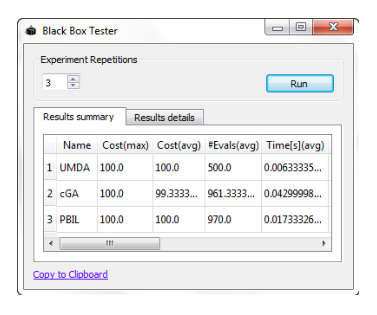
\includegraphics[scale=1.1]{onemax_bbsummary}
	\label{fig:onemax1}}
	\subfigure[]{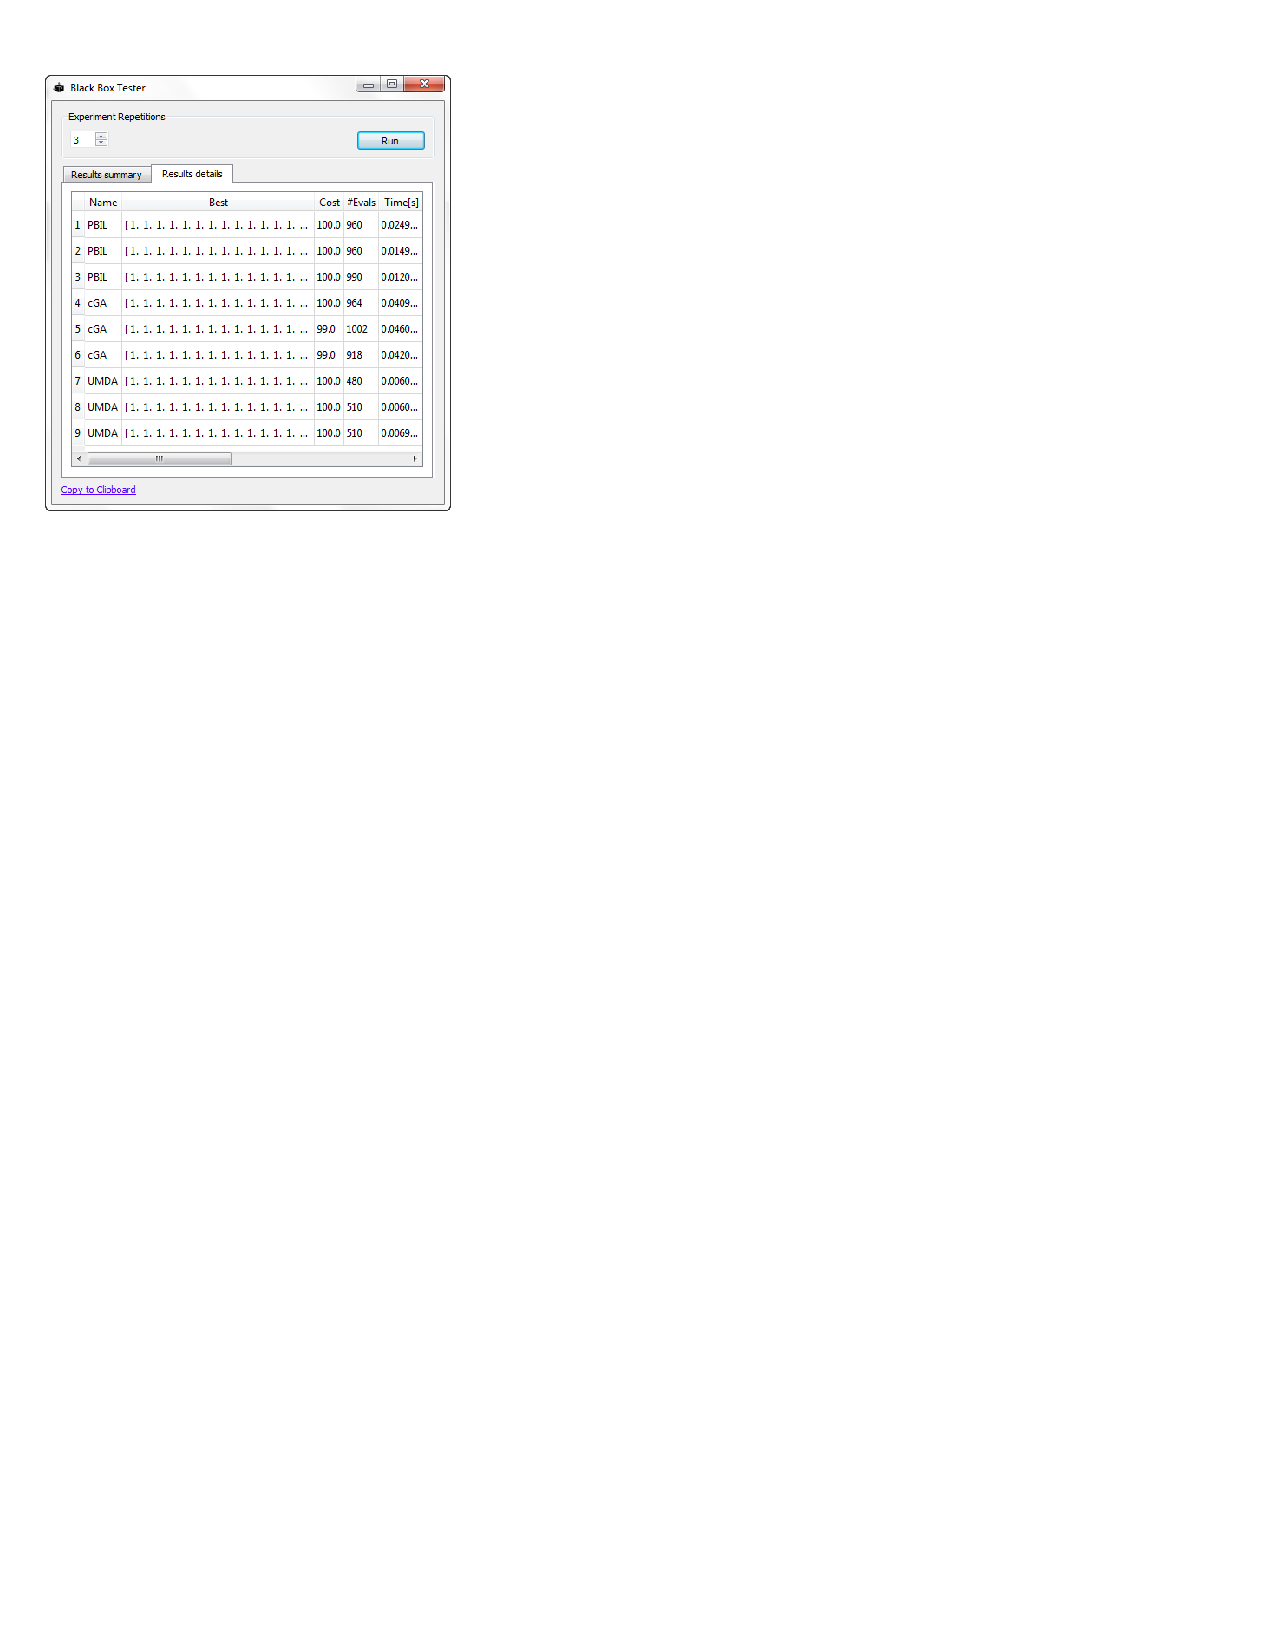
\includegraphics[scale=.95]{onemax_bbdetails} 
	\label{fig:onemax2}}
	\caption{\texttt{Onemax} experiment results: \subref{fig:onemax1} Summary over all repetitions (partial view); \subref{fig:onemax2} Details per repetition (partial view).}
	\label{fig:onemax}
\end{figure}

\subsection{Benchmark function optimization}
Two problems were chosen from the built-in benchmark library of functions: \texttt{Onemax} and \texttt{LeadingOnesBlock}. Results for the \texttt{Onemax} experiment are reported in \figref{fig:onemax}. \figref{fig:onemax1} shows the following aggregate results per \EDA~algorithm: maximun cost found in all experiment repetitions; average cost over all repetitions; average number of cost function evaluations per repetition; and average CPU time per repetition (in seconds). Other statistics can be displayed by scrolling the table bar to the right. Notice that the obtained tabulated results can be exported to spreadsheet software tools for further analysis by using the ``Copy to Clipboard'' option located underneath the output table. \figref{fig:onemax2} shows a detailed view of the results obtained in the experiments. Here each row holds the outputs per repetition for each input \EDA~component. The summarized results are statistics of these individual records. The only column not used in the summarized report is the actual vector representation of the best solution found in each run (for \texttt{Onemax} the expected solution is an all-ones vector). The cost of this solution is shown in the next column to its right.  

For the \texttt{LeadingOnesBlock} experiment, results are similarly self-explained, as reported in \figref{fig:onesblock}.

\begin{figure}[H]
	\centering
	\subfigure[]{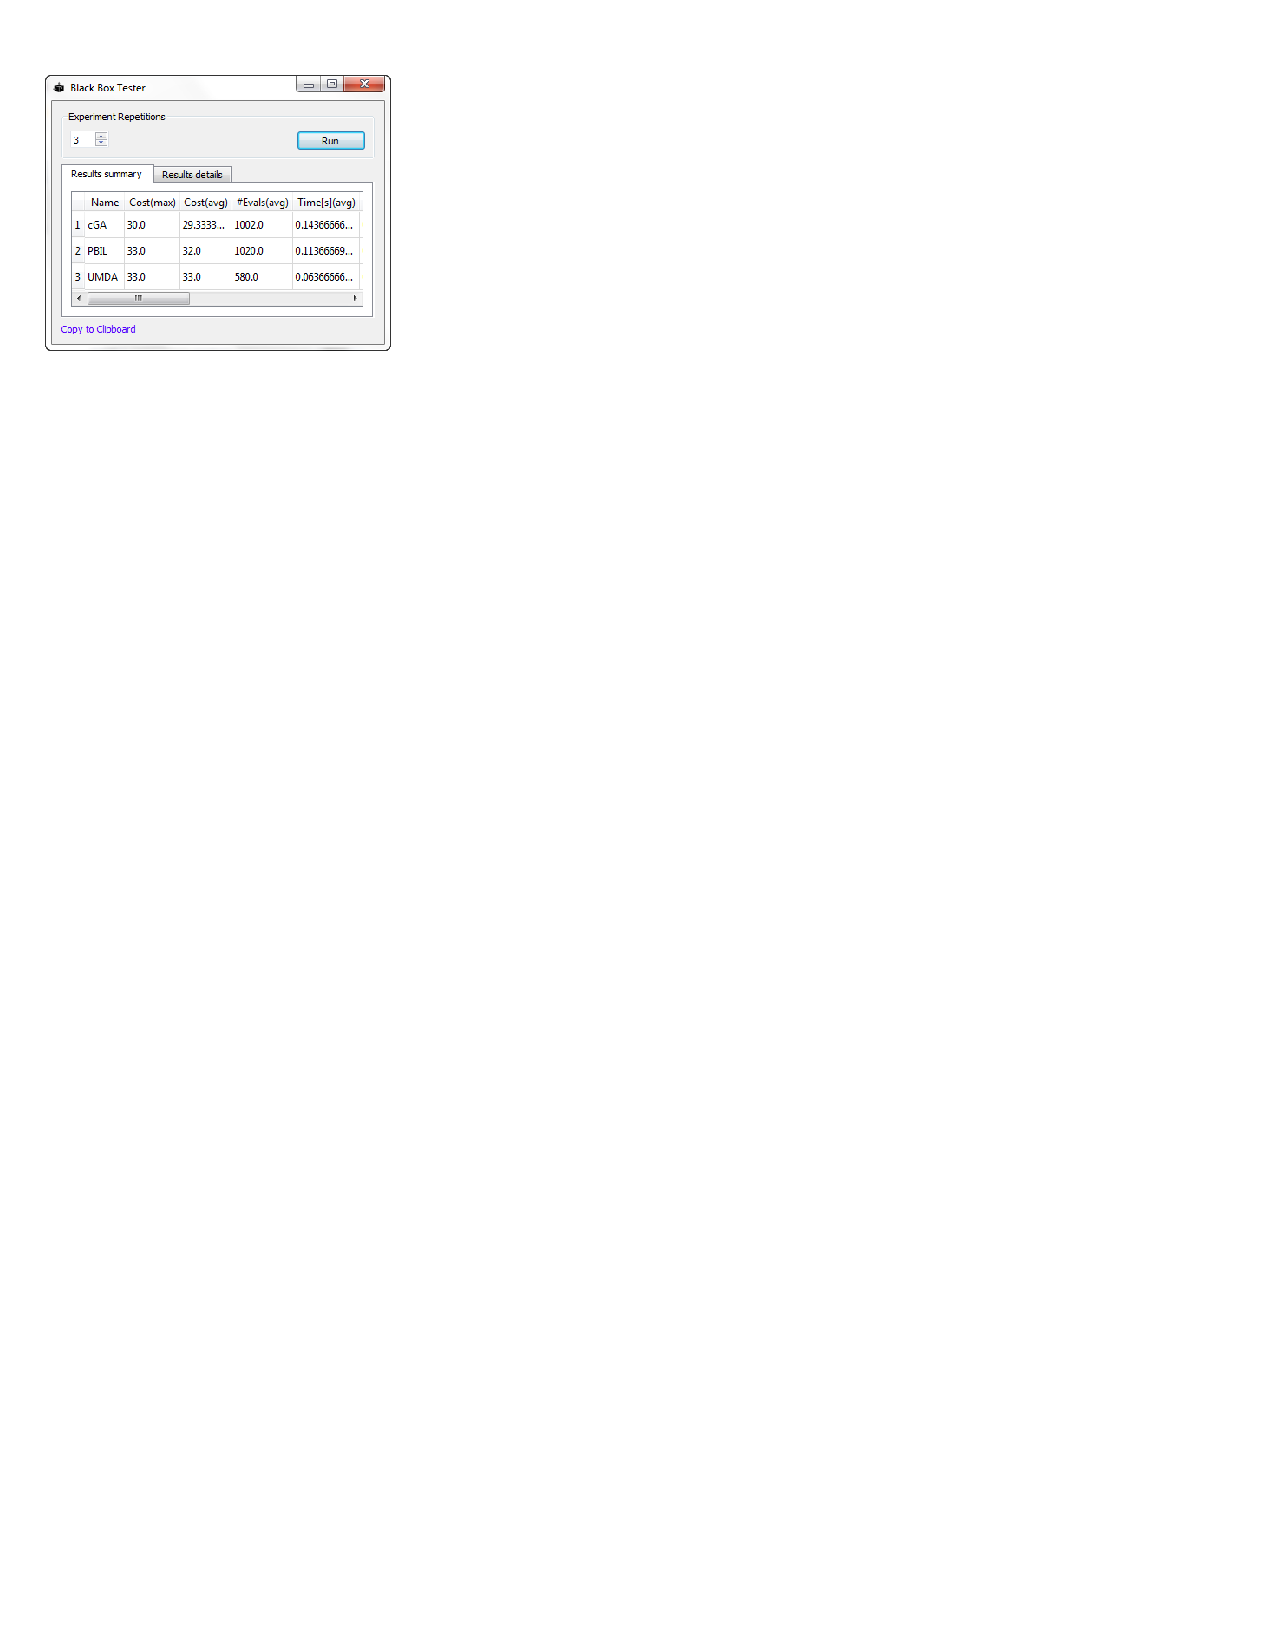
\includegraphics[scale=1.1]{onesblock_bbsummary}
	\label{fig:onesblock1}}
	\subfigure[]{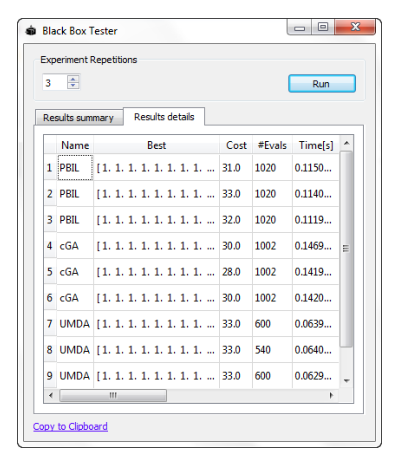
\includegraphics[scale=.9]{onesblock_bbdetails} 
	\label{fig:onesblock2}}
	\caption{\texttt{LeadingOnesBlock} experiment results: \subref{fig:onesblock1} Summary (partial view); \subref{fig:onesblock1} Details  (partial view).}
	\label{fig:onesblock}
\end{figure}


\subsection{Customized function optimization}
In this experiment we used the same \GB~program of \figref{fig:canvas} to carry out optimization of the customized cost function defined in \figref{fig:custom_costfun}, that is, the same \texttt{Leading\-OnesBlock} problem this time with a \texttt{block\_size} value of $10$. Similarly to the other experiments, results are shown in \figref{fig:custom}. 

\begin{figure}[H]
	\centering
	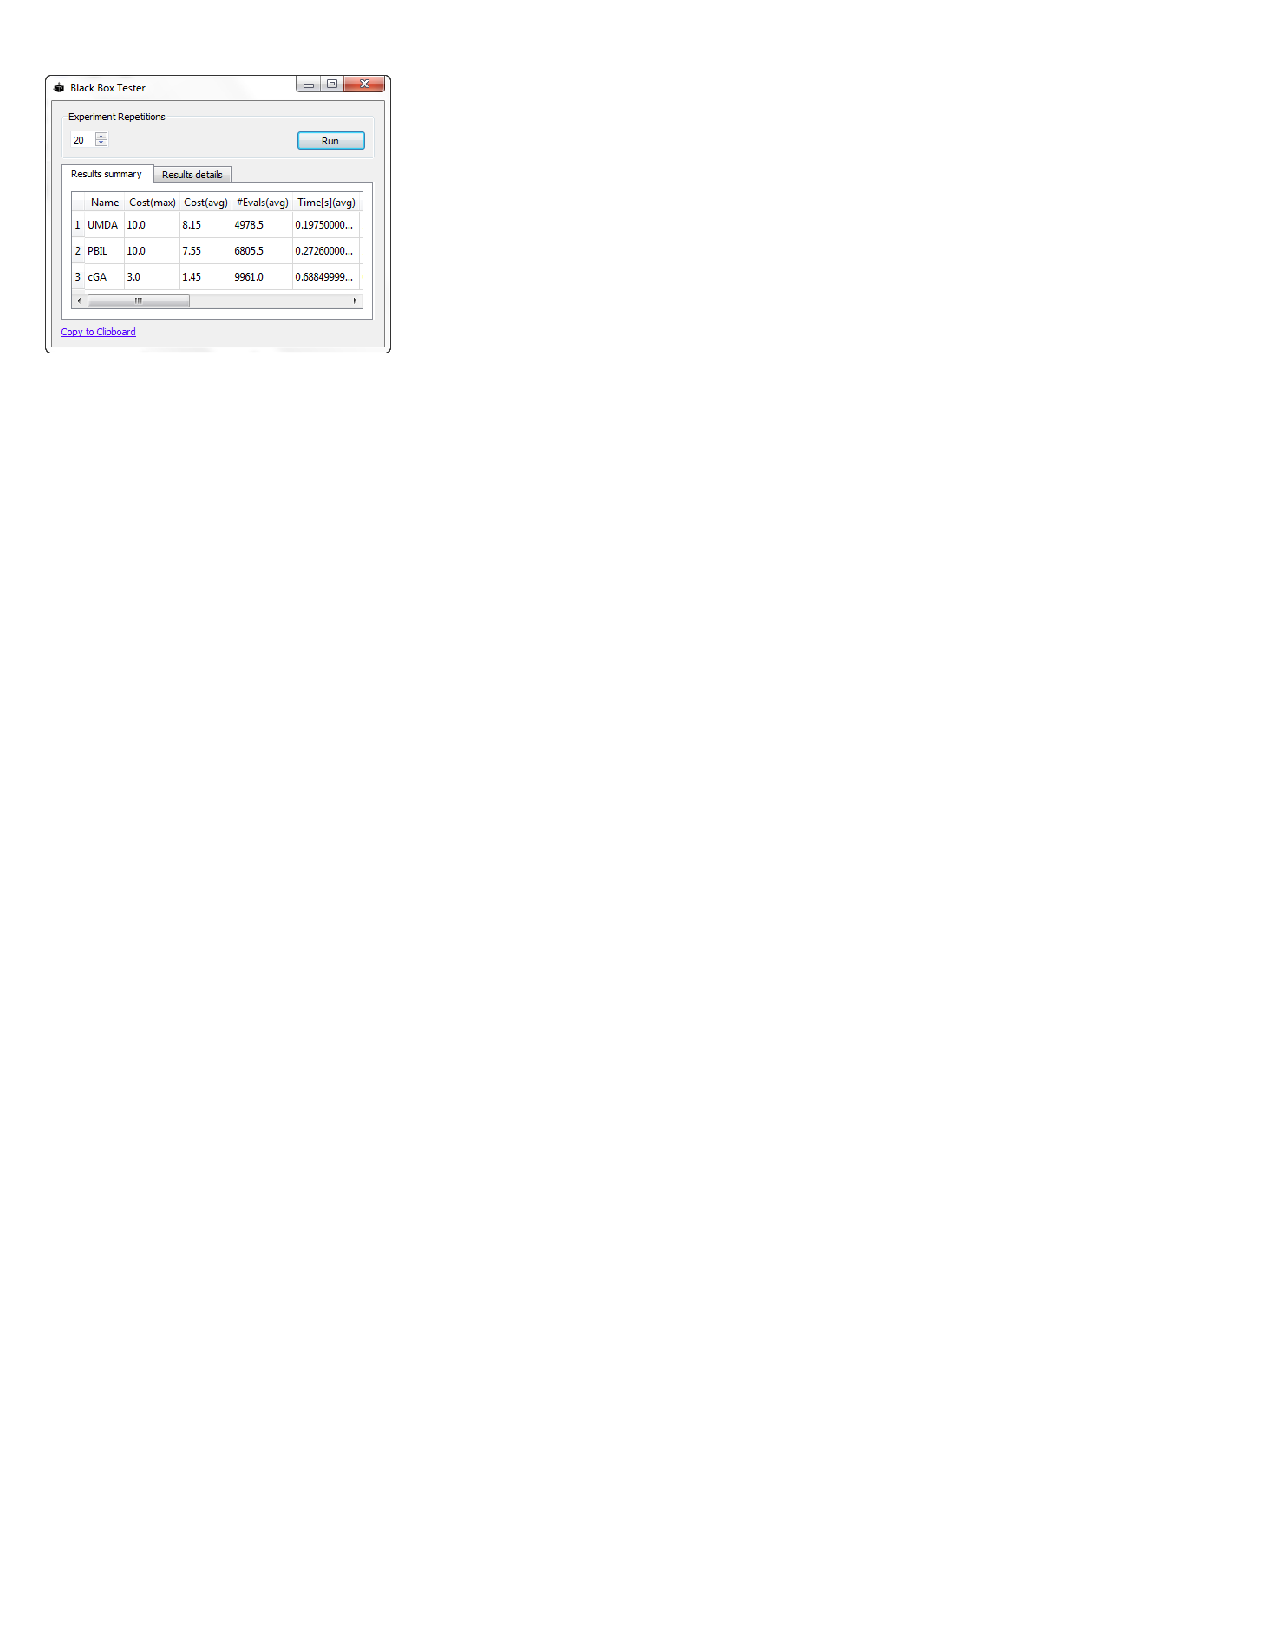
\includegraphics[scale=1]{custom_bbsummary} 
	\caption{Results of custom function experiment.}
	\label{fig:custom}
\end{figure}

\section{Conclusions}
\label{sec:conclusions}

It is our belief that user-friendly, open-source visual tools may have a big potential benefit in tasks carried out daily by data mining analysts. The \Orange~platform is a fantastic effort complying with these premises by combining a powerful visual programming approach with the reuse and glue principles of component-based software. The \GB~initiative is a modest contribution intended to extend the application domain of \Orange~to the field of black-box and metaheuristics optimization. In this first release we developed a number of \EDA-based software components featuring a non-intrusive, runtime-binding interface to allow users to define tailor-made discrete and continuous optimization problems. 

As it was mentioned in the introduction, it is anticipated that these components can be used independently as function optimizers, as it is reported in this paper, or as part of higher-level data mining machines. Let us illustrate the point with the task of feature selection. The aim there is to select an optimal subset of relevant variables for a classification problem; the relevant found subset can be further analysed by experts for specific purposes (in biology for example, features may represent over-expressed gene activity due to an illness condition). In the so-called \textit{wrapper} scheme of the problem \cite{Saeys2007} the classifier is enabled to incorporate the selection mechanism during the learning stage: a weighted kernel classifier, for example, may use an \UMDA~component to define relevance coefficients for the variables and then use them as input for the kernel machine (that is the approach taken in \cite{Rojas2008}). Currently these type of mechanisms are hidden in the current implementation of classifier or clustering components of \Orange. Thus, by providing interfaces to black-box optimizers we hope to extend applicability to this type of tasks, giving researchers a flexible workbench to design new component-based machine learning techniques. Novel components complying with the design principles described in this paper will be needed though (e.g. component-based genetic algorithms, kernel machines, etc.), and that would be matter of the next \GB~release.

%As a closing remark, this effort hopes to call for the attention of enthusiasts and practitioners in the evolutionary computation community, and also to grow their interest in using and contributing to this kind of software tools.

\section{Acknowledgements}
We would like to acknowledge Henry Diosa, Leidy Garz\'on and Harry Sanchez, members of the Arquisoft Research Gro\-up from the District University of Bogota, for the design and implementation of the \BBTester~component. We also thank the anonymous reviewers for their valuable comments which allowed us to greatly improve readability of the paper.

\bibliographystyle{abbrv}
{\scriptsize
\bibliography{biblio}  
}

\section*{Appendix. Download and installation}
\GB~is hosted publicly under a GPL license in Codeplex (\texttt{http://goldenberry.codeplex.com}). To install the software follow these steps:
\begin{enumerate}
\item Download and install Orange 2.6.1 from:\\ \texttt{http://orange.biolab.si/download/}.
\item  Get the latest \GB~release from the \texttt{Downloads} tab in \texttt{http://goldenberry.codeplex.com} (the download link is located to the left side of the screen).
\item  Follow the installation instructions in the release notes just below the download link.
\item  Open the \Orange~application and look for the ``Optimization'' toolbar in the canvas (as shown in \figref{fig:canvas}).
\end{enumerate}

%\begin{figure}[H]
%	\centering
%	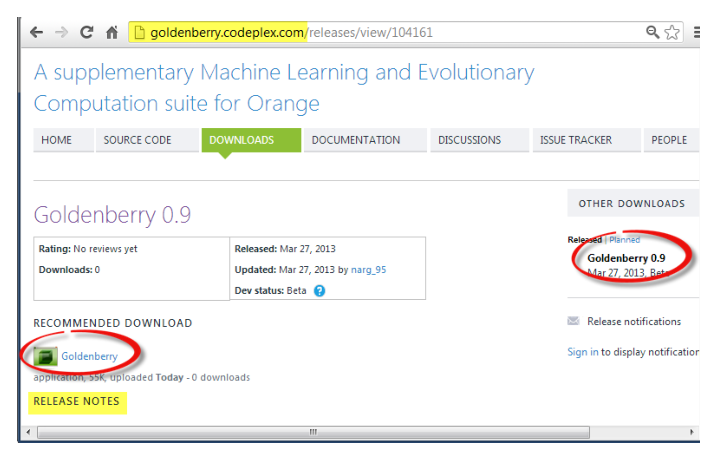
\includegraphics[scale=.75]{website_download} 
%	\caption{Snapshot of the \GB~webpage.}
%	\label{fig:website_download}
%\end{figure}

%\begin{figure}[H]
%	\centering
%	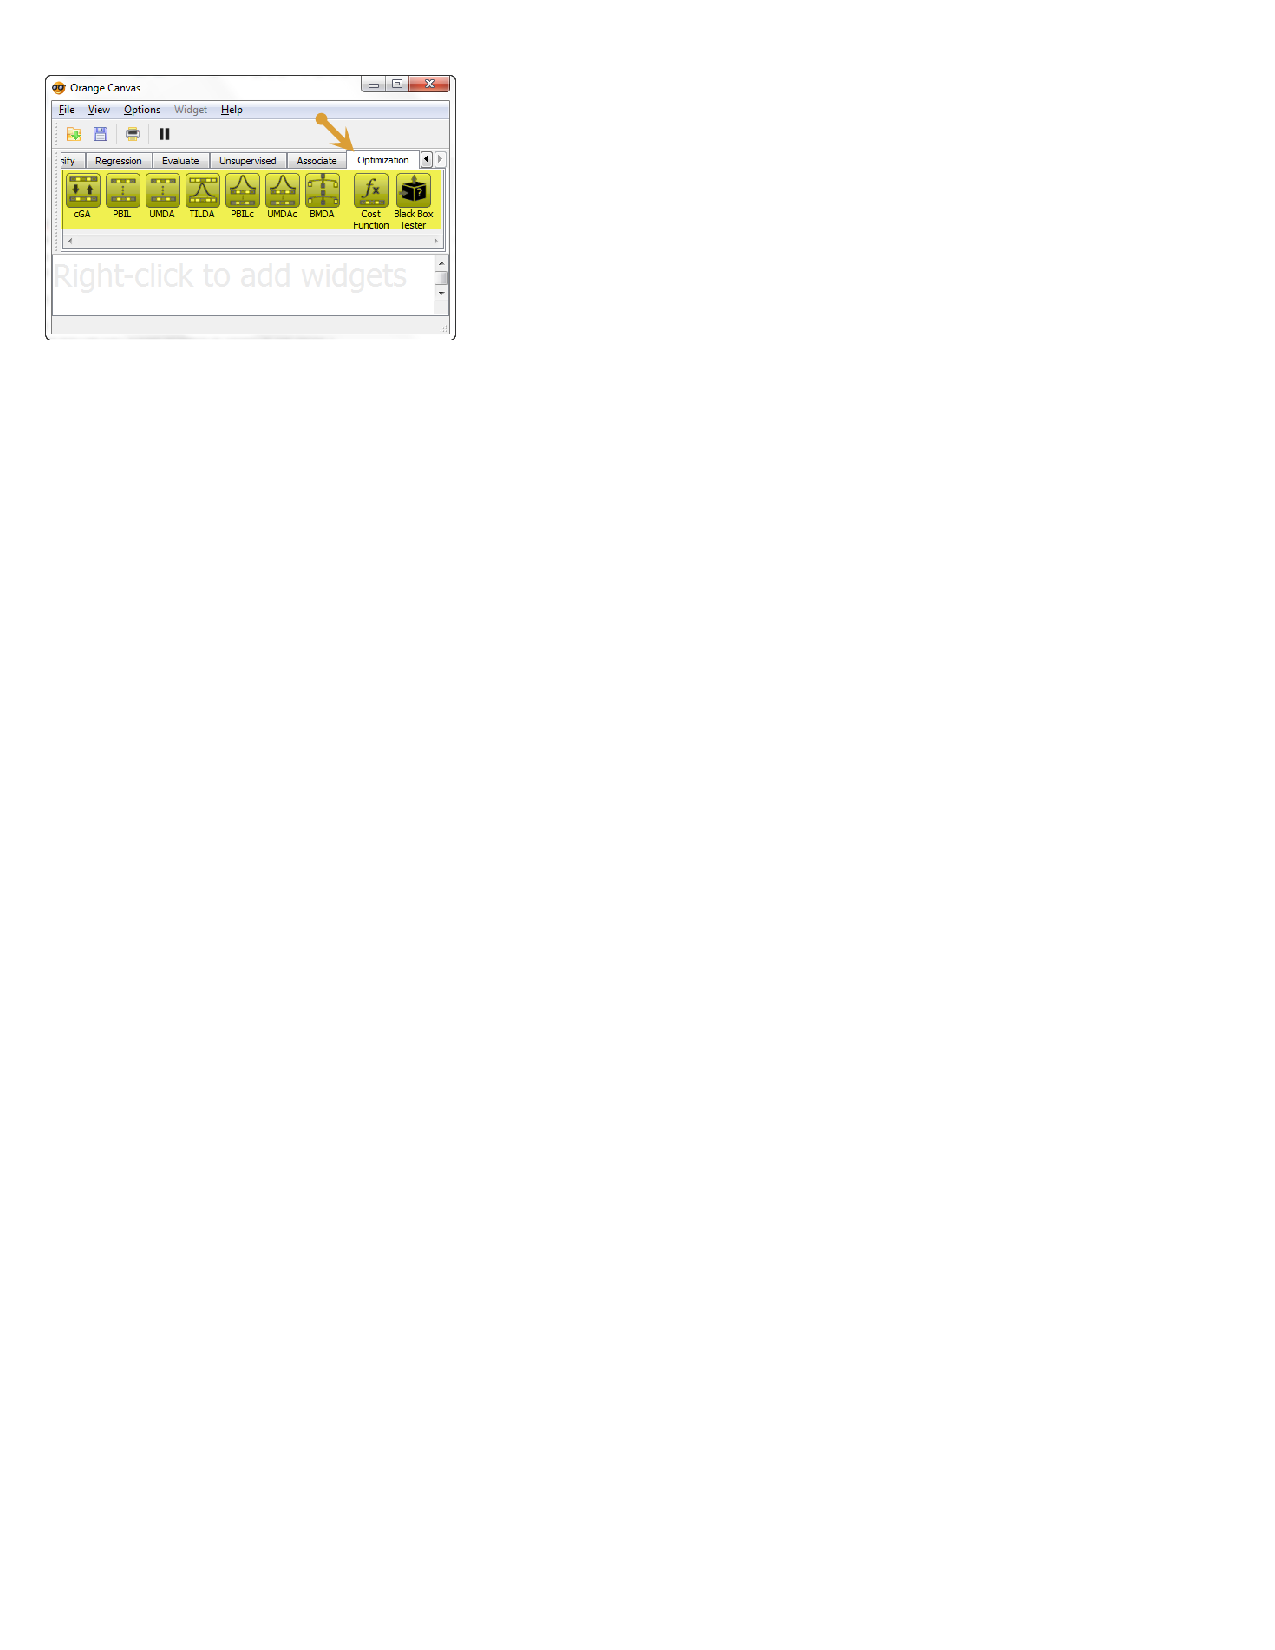
\includegraphics[scale=1]{install_toolbar} 
%	\caption{The \GB~toolbar in \Orange.}
%	\label{fig:install_toolbar}
%\end{figure}

\vfill
\end{document}
